% !TEX encoding = UTF-8 Unicode

Durante a parte de especificação da segunda prova, a etapa 2, escolhi especificar toda a estrutura da linguagem \emph{SimpPro} dentro da memória do \emph{RNA}, com a inferência sendo executada pelo interpretador \emph{RNA}. Porém, ao observar que a variável \textbf{strg} só possuía 1 Byte, só seria possível acessar 256 células de memória, o que poderia complicar a implementação do motor de inferência no \emph{RNA}.

A partir dessa constatação, decidi implementar a geração de novos fatos a partir dos fatos originais e das cláusulas no C, de forma progressiva, sem observar a meta desejada. Com a inferência completa, foi adicionado a fita do \emph{RNA} somente a meta e a base de fatos completa, além do código que busca a meta na lista de fatos e retorna se encontrou ou não.

Foram criadas 11 ações semânticas, adicionadas no autômato em diferentes posições e exibidas na Figura~\ref{fig:semantico}.

\begin{figure}[htbp]
    \centering
    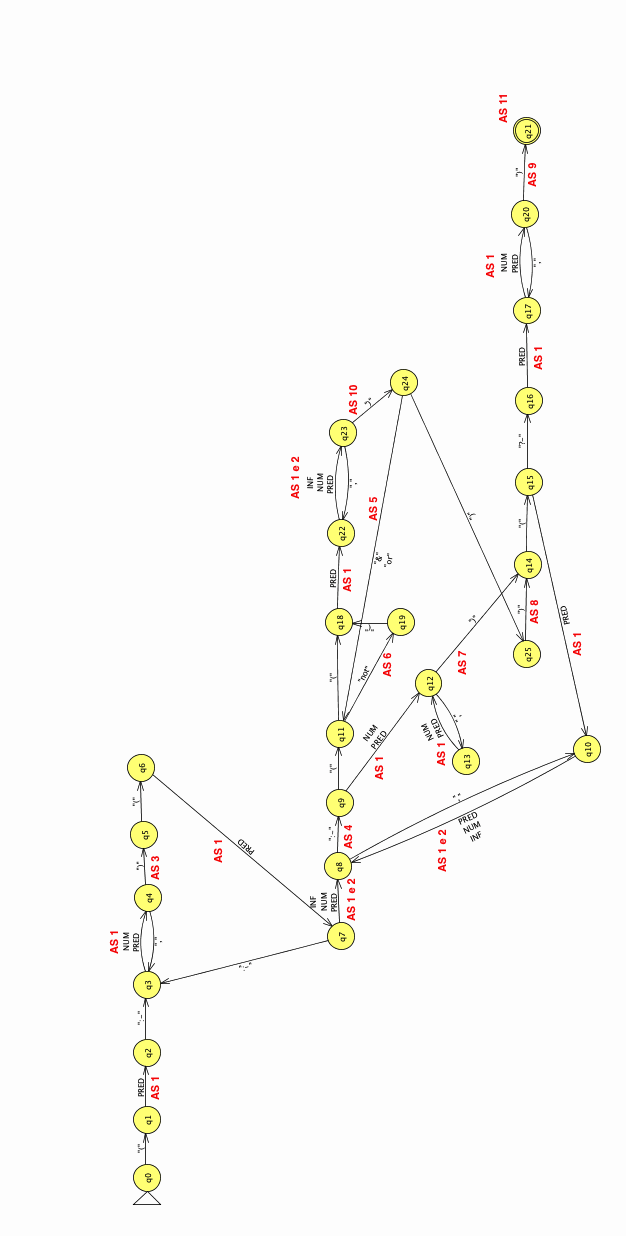
\includegraphics[width=0.75\textwidth]{./images/semantico.png}
    \caption{Autômato \emph{Program} com ações semânticas}
    \label{fig:semantico}
\end{figure}

A breve descrição das ações semânticas implementadas está listada abaixo:

\begin{enumerate}
	\item \textbf{AS 1}: Insere a constante (PRED ou NUM) na lista de constantes.
	\item \textbf{AS 2}: Insere a variável (INF) na lista de variáveis.
	\item \textbf{AS 3}: Insere o fato na lista de fatos.
	\item \textbf{AS 4}: Insere a parte esquerda da cláusula na lista de sentenças e adiciona a referência da sentença na cláusula a ser processada.
	\item \textbf{AS 5}: Insere o operador lido (``\&'' ou ``or'') na cláusula a ser processada.
	\item \textbf{AS 6}: Insere o operador not na cláusula a ser processada.
	\item \textbf{AS 7}: Ação que trata a operação (avo joao, maria :- jose, joaquim, 3), cláusulas que tem dados na parte direita da sentença. Como acordado com o professor, não será implementado por não ter correspondência com o resultado que é verdadeiro ou falso.
	\item \textbf{AS 8}: Insere a cláusula já construída nas outras ações na lista de cláusulas.
	\item \textbf{AS 9}: Insere a sentença lida como meta. Também chama o motor de inferência que gera os fatos inferidos a partir das cláusulas e dos fatos originais.
	\item \textbf{AS 10}: Insere a sentença formada previamente na lista de sentenças e adiciona a referência da sentença na cláusula a ser processada.
	\item \textbf{AS 11}: Ao terminar de ler o programa corretamente, chama a geração de código que escreve em \emph{RNA} a meta, os fatos gerados e o código necessário para verificar se a meta está contida na lista de fatos e imprimir 1 para verdadeiro ou 0 para falso.
\end{enumerate}

A geração de código foi efetuada através de uma estratégia que facilitou bastante o processo de criação dos algoritmos em \emph{RNA}. Eu desenvolvi um conversor em C++ de C para RNA e de RNA para C, utilizando a descrição dos comandos disponibilizada na Wiki da linguagem e mostrado no Capítulo~\ref{chap:linguagem-rna}. O conversor está presente no código anexado, na pasta ``rna/testes/conversor.cpp''. Com esse conversor, desenvolvi os códigos a serem gerados em C e converti ao final para \emph{RNA}, copiando o código gerado dentro do compilador. Cabe ressaltar que o conversor também foi crucial para entender e \emph{debugar} o código \emph{RNA} gerado durante o desenvolvimento.
